\section{Svolgimento}
\subsection{Analisi del problema}
Abbiamo iniziato analizzando le richieste del problema da un punto di vista matematico. Per risolverle, bisogna essere in grado di trovare i documenti che contribuiscono all'incremento del fatturato e discriminare gli altri. In un secondo momento, è necessario calcolare la media (Eq.\ref{eq:media}) e la varianza (Eq.\ref{eq:varianza}) utilizzando le formule sottostanti.
\begin{equation}
    \bar{x} = \frac{1}{n} \sum_{i=1}^{n} x_i
    \label{eq:media}
    \end{equation}
    
    \begin{equation}
    \sigma^2 = \frac{1}{n} \sum_{i=1}^{n} (x_i - \bar{x})^2
    \label{eq:varianza}
    \end{equation}
    
Successivamente, sarà necessario calcolare l'ammontare del fatturato diviso per ogni mese di ogni anno. Una volta elaborate queste informazioni, si può procedere ad identificare il mese di ogni anno che ha il valore più alto e più basso, analizzandoli tramite le funzioni di minimo e massimo e raggruppando per anno.
\subsection{Analisi del Dataset}
Procediamo con l'analisi del dataset con i comandi
\begin{lstlisting}[language=R]
    summary(df)
    table(df$tipo)
\end{lstlisting}
che vengono utilizzati per valutare la tipologia dei dati e per estrarre i valori della prima colonna riferiti al tipo di documento.
\begin{table}[ht]
\centering
\begin{tabular}{|l|c|}
\hline
Tipo di documento & Quantità \\
\hline
BUONO.PRELIEVO & 2146 \\
DDT & 15 \\
FATTURA & 556 \\
INVENTARIO & 1 \\
NOTA.DI.CREDITO & 9 \\
OFFERTA & 622 \\
PREVENTIVO & 240 \\
RICEVUTA & 11 \\
\hline
\end{tabular}
\caption{Analisi delle tipologie di documento}
\label{tab:esempio}
\end{table}
In prima analisi, ci rendiamo conto che i documenti che apportano incremento al fatturato sono della tipologia fattura e ricevuta. Andiamo quindi ad impostare un filtro che ci aiuta ad estrarre dal dataset i documenti interessati.
\subsection{Risoluzione tramite codice R}
A questo punto, procediamo con il calcolo della media utilizzando la funzione \codeword{aggregate}, aggregando in base ai mesi di ogni anno e applicando la funzione di calcolo della media (\codeword{FUN = mean}). Vengono fatti in seguito delle trasformazioni per estrarre dalla data le informazioni di anno e mese e renderle più facilmente leggibili. Successivamente, andiamo a calcolare la varianza utilizzando la stessa funzione \codeword{aggregate} e impostando \codeword{FUN = var}.


\begin{figure}[ht]
\centering
\begin{minipage}{.3\textwidth}
    \centering
    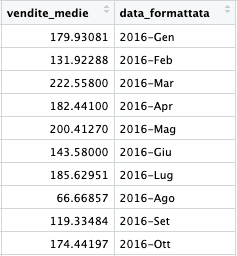
\includegraphics[width=\linewidth]{img/media_r.png}
    \caption{Estratto del dataset con la media}
    \label{fig:immagine1}
\end{minipage}
\begin{minipage}{.3\textwidth}
    \centering
    \end{minipage}
\begin{minipage}{.3\textwidth}
    \centering
    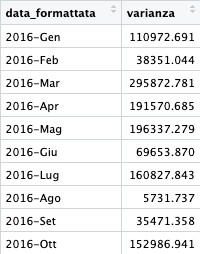
\includegraphics[width=\linewidth]{img/varianza_r.png}
    \caption{Estratto del dataset con la varianza}
    \label{fig:immagine2}
\end{minipage}
\end{figure}
Per la soluzione dei job 3 e 4, si è reso necessario andare a fare un calcolo preliminare, ovvero aggregare le informazioni delle vendite in base al mese e all'anno. Successivamente, si è estratto il valore maggiore (per il job 3) e il valore minore (per il job 4) e visto che si è persa l'informazione specifica del mese, è stato necessario andare a recuperarla facendo un merge con la tabella aggregata precedente e le due tabelle risultanti dall'estrazione dei valori di minimo e massimo.
\begin{lstlisting}[language=R]
    mesi_max = merge(mesi_max_solo_anno, somma_mesi, by="vendite_totali")
\end{lstlisting}
\subsection{MapReduce usando Javascript}
Una volta affrontato il problema con lo scritto in R, andiamo ad analizzare il problema sotto il paradigma di MapReduce. Per una prima analisi, utilizziamo lo strumento del professor Pirrone che permette un rapido approccio a questo modo di scrivere codice. I primi step intrapresi sono andare a dividere il file di input per riga e darlo in pasto allo script di mapping.
La fase di mapping prevede la divisione della linea letta in input e sui tre valori che porta (tipologia ordine, data e costo). Successivamente, andiamo (come fatto in precedenza) a filtrare per la tipologia di ordine fattura e ricevuta: nel caso in cui la tipologia d'ordine appartenga a queste due categorie, viene creata una coppia che ha come chiave la data e come valore l'importo, o costo, del documento.


\begin{lstlisting}[language=Java, caption={Script di mapping}]
    return V_In_Map.map(function(item){
        //scrivo il codice di map
        var tipoOrdine = item.split(",")[0]
        var data = item.split(",")[1]
        var costo = item.split(",")[2]

        var chiave;
        var valore;
        if(tipoOrdine === "FATTURA" ||
        tipoOrdine === "RICEVUTA"){
            chiave = data.slice(0,6);
            valore = costo;
        }
        else
        {
            chiave = "NULL";
            valore = 0;
        }
        return keyVal(chiave, valore);
    });

\end{lstlisting}
Serve fare una precisazione: in un paradigma di MapReduce normale, è possibile scartare dei dati in input. In questo tool, è sempre necessario fornire un output di mapping. Di conseguenza, invece di scartare i documenti che non sono utili al fine del programma, vengono mappati con una chiave "null", che nelle elaborazioni successive non verrà considerata.

Per il primo job, lo script di reduce andrà a recuperare tutti i valori relativi ad una determinata chiave, ovvero ad una data, e a calcolare la media (andandoli a sommare e successivamente a dividere per il numero di valori associati a quella data).

Nel secondo job, andiamo a riciclare lo stesso script di mapping. Per la fase di reduce, andiamo prima a calcolarci la media di valori associati a quella data (esattamente come il job precedente). Il secondo passaggio è quello di andare a calcolarci per ogni valore lo scarto quadratico rispetto alla media, utilizzando la formula (Eq.\ref{eq:media}, Eq.\ref{eq:varianza}).